\chapter{Framework Application for Design}
\label{chapter:application}

To verify that the conceptual framework is effective, I applied it to design a place photo discovery application. This chapter outlines the role the framework played in the design process of the Web application, the resulting application and its features, and some prospects for future application development. 

{\section{Applying the Conceptual Framework to Design an Application}
A need for a place photo discovery application was revealed during the construction phase of the framework. Asking questions from the preliminary framework (see Chapter~\ref{chapter:old_framework}) about existing applications, such as Pinterest and Google Maps, helped expose the need for discovery and curation of place photos with additional access to place location data and other details. It also helped gather some of the requirements for a photo discovery application. Once user needs and motives for information discovery and curation of place photographs where established, I repeatedly consulted the framework throughout the development process of the application in order to systematically select the next feature to be implemented.

In general, Web applications that are tailored towards image discovery, such as Pinterest and We Heart It, support user's motive to close a knowledge gap that is characterized by underdefined information needs. To deal with the issue of having an underdefined information need, an application has to help the user to formulate their information need as well as support serendipitous discovery of information. In order to enable serendipitous discovery, Web applications regularly update the content they provide by allowing users to add new resources and curate information. 

The task of image seeking for the purpose of finding inspiration (as it is the case for the majority of Pinterest users) can stretch out to multiple sessions over an undetermined period of time. Curation mechanisms, such as preservation and management, help the user to rediscover information that allows them to reflect on the previous findings and continue image seeking.  

It is common for users to discover place photographs on Pinterest, and Pinterest does display a map when a location of a place is known within the system. However, this feature only applies to a relatively small fraction of existing `pins'. In addition, Pinterest facilitates discovery of images related to diverse topics and interests, and not only places, which makes it harder to tailor the user experience to facilitate discovery and curation based on their desired motives. 

When it comes to place discovery, the Google Maps application provides the ultimate support for finding place and business locations. It is also possible to see what a place looks like based on an associated image. However, since the application is oriented towards finding specific information, visual and spatial photo exploration mechanisms are not well-developed. The user can preserve a given place but cannot preserve or organize photographs of places. Google Maps also lacks category-based navigation mechanisms which can help the user identifying their information needs.  

The findings above helped me define a motive for a place photo discovery application, which is \textit{to find inspirational (underdefined) place photographs, to collect and manage found information for future use and retrieval, as well as to provide access to more defined information about the place}, such as its location. After formalizing the motive for the application use, I refer back to the framework to choose options for supporting various aspects of information discovery and curation while developing the application.
}

{\section{KeePlaces Features and Future Prospects}
The resulting Web application, KeePlaces\footnote[1]{A prototype of KeePlaces is available at www.keeplaces.com} (see Figure~\ref{fig:keeplaces}), supports discovery and curation of place photographs, and it is integrated with Google Maps. This section outlines the main features of KeePlaces in accordance with the conceptual framework (see Appendix~\ref{chapter:appendix_keeplaces}). 

KeePlaces supports descriptional, referential, and partially system-regulated navigation methods. It is possible to perform descriptional navigation using \textbf{integrated search} that in turn utilizes Google Maps APIs to search for photographs of different places. The search feature is not \textbf{guided}, and at this time, results are not \textbf{personalized}. Descriptional navigation could be improved by suggesting search terms to the user once they start typing. However, personalizing the results of searching might not be a good strategy because users might want to explore photographs that they have not seen before or that are of places not related to them. 

Users can navigate using \textbf{categories} which enable referential navigation. Currently, categories that users might be interested in are only approximately estimated, and no other traditional referential mechanism is employed for navigating within the application. However, the users can navigate to Google Maps by clicking "View Google Maps" link beside every photograph to see where the place is located and perform any other actions within the Google Maps application. This feature enables \textbf{integrated referential navigation}. 

With the preliminary prototype, as the user first visits KeePlaces, the system displays predefined tourist attraction photographs, and therefore, it supports system regulated navigation by displaying \textbf{featured content}. However, this solution is temporary since system-regulated navigation could be further improved by \textbf{personalizing featured content} and delivering \textbf{notifications} about content updates to the user. 

Currently, \textbf{opportunistic navigation} is not enabled in KeePlaces although users with undefined information needs could benefit from this method. Alternatively, other navigation methods could return serendipitous results.

Spatial exploration of multiple resources is enabled using \textbf{gallery layout}. A \textbf{grid layout} could be an alternative way to present information within the application; however, \textbf{list} is not always an optimal solution to presenting visual data. 
Resources are represented as photographs, and these photographs serve as \textbf{visual cues} to what the places they represent look like. In addition to visual cues, \textbf{textual cues} provide names of different places delivering additional exploration support.

KeePlaces does not support exploration of individual resources as of today; however, enabling it could improve future information discovery. Furthermore, allowing users to \textbf{personalizate} of visual or textual cues can help them rediscover place photographs and collections. 

\pagebreak

Curation in KeePlaces is supported through management and preservation. Management is implemented using \textbf{collection-based classification}.
Every photo discovered on the site can be bookmarked by clicking the the `Keep' button and choosing a collection. This bookmarking mechanism enables \textbf{internal preservation of internal resources} since it allows to save information found within KeePlaces. 

Some aspects of curation, such as information sharing, augmentation, and channel-picking have not been enabled yet. These activities are important because they contribute to collaborative and creative environments as well as help building community around the Web application. In KeePlaces, having the users add new photographs and share them among themselves could scale the application usage up and enrich the quality of the content provided to the users. 

In order to support channel-picking, a Web application must regularly update its content, which can be done by either moderators or general users. Then, adding \textbf{subscription mechanisms} and \textbf{notifications} can further empower channel-based discovery.  For place photo discovery, a tool, such as KeePlaces, can provide updates about photographs preserved by other users, new photographs added to the pool of information, spatial featured photographs, etc.

Although KeePlaces has not been released as a stable Web application yet, it supports the discovery and curation of place photographs from all over the world. Applying the framework above as presented, can guide its future development and evaluation.  

\begin{figure}[ht!]
	\noindent
	\centering
	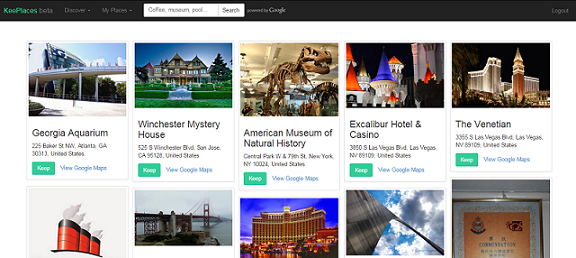
\includegraphics[width=\linewidth]{keeplaces.png}
	\caption{KeePlaces Interface}
	\label{fig:keeplaces} 
\end{figure}

} % end section

{\section{Discussion}
The conceptual framework for information discovery and curation guided the design of the place photo discovery application, KeePlaces. The framework assisted in identifying the need for a Web application that facilitates the discovery of place photographs in particular, and it highlighted which design elements are important in this specific case. Similarly, the framework can aid in the design process of other applications. 

When the motive for an application use is known, one can evaluate Web applications from similar domains to identify gaps in the provided features. Finding feature gaps is a challenging task, but the framework can assist by making easier to relate relevant information behaviour with concrete mechanisms and features. Ongoing reevaluation of the tool and its competitors using the framework can help with continuous development process and improve user experience when they interact with the system.
} % end section




